\hrulefill 
\section{Sprint 2}

\subsection{Goal}
L'obiettivo di questo secondo sprint è stato quello di migliorare la grafica, User Interface, per presentare, attraverso un video, al comune una prima idea di come potrebbe presentarsi la nostra web app.
Inoltre abbiamo puntato a migliorare la gestione degli account attraverso i token firebase e l'inserimento dei differenti ruoli che un utente può avere: Cliente e Produttore assegnati durante la registrazione e il ruolo Amministratore ottenibile solo attraverso l'inserimento manuale nei vari database utilizzati.

Oltre a questi due goal abbiamo anche implementato la gestione del recupero password, la gestione del carrello e l'inserimento, cancellazione e modifica di un prodotto nell'interfaccia fornita al produttore.

\subsection{Sprint Planning}

% \subsubsection{Tabella sprint backlog}

\vspace{-1cm}

\renewcommand{\arraystretch}{2}
\begin{longtable}{p{0.5cm}|p{2.7cm}|p{4.5cm}|p{1.7cm}|p{1.5cm}|p{0.2cm}|p{0.2cm}|p{0.2cm}|p{0.2cm}|p{0.2cm}|p{0.2cm}}
    \caption{Tabella sprint backlog}
    \label{tab:SprintBackLogTableDettagliato} \\
    
    \hline
    \textbf{ID} &\textbf{Nome} & \textbf{Sprint Task} & \textbf{Volontario} & \textbf{Impegno stimato iniziale} & 1 & 2& 3& 4& 5& 6\\
    \hline
    \endfirsthead
    
    \hline
    \textbf{ID} &\textbf{Nome} & \textbf{Sprint Task} & \textbf{Volontario} & \textbf{Impegno stimato iniziale} & 1 & 2& 3& 4& 5& 6\\
    \hline
    \endhead
    
    
    \multirow{6}{0.2cm}{14} & \multirow{6}{0.2cm}{Inserimento prodotto} 
    & creazione di una UI più complessa & Giacomo & 3 & 3& 2& 1& & & \\
    && Pagina dedicata solo a persone che si loggano come produttore & Giacomo & 2& 2 & 2& 1& & & \\
    && Verifica del token firebase lato backend & Giacomo & 1& 1 & 1& 1& 1& & \\
    && Creazione di un nuovo endpoint di risorsa annidato & Giacomo & 3& 3 & 3& 1& 1& & \\

    
    \hline    
    \multirow{3}{0.2cm}{15} & \multirow{3}{0.2cm}{Rimozione prodotto} 
    & Verifica del token firebase lato backend & Giacomo & 1& 1 & 1& 1& 1& & \\
    && Creazione di un nuovo endpoint di risorsa annidato & Giacomo & 1& 1 & 1& 1& 1& & \\
    
    
    \hline
    \multirow{3}{0.2cm}{20} & \multirow{3}{0.2cm}{Aggiornamento prodotto} 
    & Verifica del token firebase lato backend & Giacomo & 1& 1 & 1& 1& 1& & \\
    && Creazione di un nuovo endpoint di risorsa annidato & Giacomo & 1& 1 & 1& 1& 1& & \\
    
    
    \hline
    
    \multirow{2}{0.2cm}{2} & \multirow{2}{0.2cm}{Autenticazione cliente/produttore } 
    & creazione di una UI più complessa & Martina & 2 & 2& 1& & & & \\
    % && inserire il bottone di autenticazione con Google & Martina & 4&4 & 3& 2& 1& & \\
    \hline
    
    \multirow{2}{0.2cm}{5} & \multirow{2}{0.2cm}{Ricerca prodotti} 
    & creazione di pagina frontend per la ricerca dei prodotti & Cristiano & 1 & 1& & & & & \\
    && aggiungere all'API di lettura prodotti la funzione di ricerca & Cristiano & 2&2 & 1& & & & \\
    
    \hline

    \multirow{2}{0.2cm}{4} & \multirow{2}{0.2cm}{Recupero password } 
    & inserire il bottone per recuperare la password & Martina & 1&1 & 1& & & & \\
    
    
    \hline
    
    \multirow{2}{0.2cm}{1} & \multirow{2}{0.2cm}{Registrazione cliente/produttore } 
    & creazione di una UI più complessa & Martina & 4 & 4& 4&3 & 2& 1& \\
    % && inserire il bottone di registrazione con Google & Martina & 4&4 & 3& 2& 1& & &\\
    
    \hline


    

    \multirow{1}{0.2cm}{16} & \multirow{1}{0.2cm}{Visualizzazione prodotti} 
    & creazione di una dashboard & Giacomo & 3 & 3& 2& 1& & & \\
    % && inserire il bottone di registrazione con Google & Martina & 4&4 & 3& 2& 1& & &\\
    
    \hline

    \multirow{3}{0.2cm}{8} & \multirow{3}{0.2cm}{Aggiunta al carrello } 
    & creazione di una sezione carrello nella UI & Martina & 4 & 4& 4& 3& 2& 1& \\
    && aggiornare i modelli del database lato backend & Martina & 4&4 & 2& 1& & & \\
    && una volta aggiunto al carrello la quantità viene scalata dal disponibile & Cristiano & 2&1 & & & & & \\
    \hline

    \multirow{2}{0.2cm}{7} & \multirow{2}{0.2cm}{Visualizza dettaglio } 
    & creazione di una card per visualizzare il dettaglio del prodotto & Martina & 2 & 2& 1& & & & \\
    
    \hline


    \multirow{2}{0.2cm}{11} & \multirow{2}{0.2cm}{Cronologia ordini } 
        & creazione di una card per visualizzare la cronologia ordini & Cristiano & 2 & 3& 2& & & & \\
    \hline


    % \multirow{3}{0.2cm}{13} & \multirow{2}{0.2cm}{Recensioni prodotti}
    % & inserimento nella UI un interfaccia che può gestire la recensione dei prodotti & Martina & 1 & 1& & & & & &\\
    % && gestire la risorsa lato bakend & Martina & 4&4 & 3& 2& 1& & &\\
    
    % \hline

    % \multirow{1}{0.2cm}{26} & \multirow{1}{0.2cm}{Gestione segnalazioni}
    % & creazione di una demo UI & Giacomo & 1 & 1& & & & & &\\
    
    % \hline

    \multirow{3}{0.2cm}{6} & \multirow{3}{0.2cm}{Ricerca produttore}
    & creazione di un componente grafico che permetta la ricerca & Cristiano & 2 & 2& 2& 1& & & \\
    && creazione di un endpoint API & Cristiano & 2 & 2& 1& & & & \\
    \hline

    \multirow{5}{0.2cm}{24} & \multirow{5}{0.2cm}{Gestione account}
    & creazione di un modello per l'amministratore lato database & Cristiano & 2 & 2 & 1& & & & \\
    && aggiunta a livello frontend della gestione del login dell'amministratore & Cristiano & 3 & 3& 2& 1& & & \\
    && aggiunta del ruolo nel token firebase & Cristiano & 2 & 2& 2& 1& & & \\
    \hline

    \multirow{5}{0.2cm}{-} & \multirow{5}{0.2cm}{Test}
    & Inizializzazione ambiente di sviluppo - Jest e superset & Cristiano & 1 & 2 & 1& & & & \\
    && Test API con Postman & Cristiano & 3 & 2& 2& 1& & & \\
    && Test API con Supertest & Cristiano & 1 & 1& 1& & & & \\
    \hline

    \multirow{5}{0.2cm}{-} & \multirow{5}{0.2cm}{Deploy applicazione}
    & Documentarsi su come funziona Render & Cristiano & 1 & 1 & & & & & \\
    && Test deploy del main (Sprint \#1) & Cristiano & 3 & 2& 2& 1& & & \\
    && Test deploy del main (Sprint \#2) & Cristiano & 1 & 1& & & & & \\
    \hline

    \multirow{3}{0.2cm}{-} & \multirow{3}{0.2cm}{Prospetto economico}
    & Compilazione piano economico & Cristiano & 1 & 1 & & & & & \\
    &  &  &  &  & & & & & \\
    \hline

    \multirow{1}{0.2cm}{-} & \multirow{1}{0.2cm}{Video}
    & Video presentazione comune & Team & 5 & 5 &4& 3& 2&1 & \\

    
    \hline
    \hline
    \hline
    \multicolumn{4}{r|}{Totale: }& 63&63&46&22&12&3&0\\
    
    \hline
    \multicolumn{4}{r|}{Ideale: }& 63&53&42&32&21&11&0\\
    
    

\end{longtable}
\restoregeometry

\newpage
\subsection{Burndown Chart}

\begin{figure}[!ht]
    \centering
    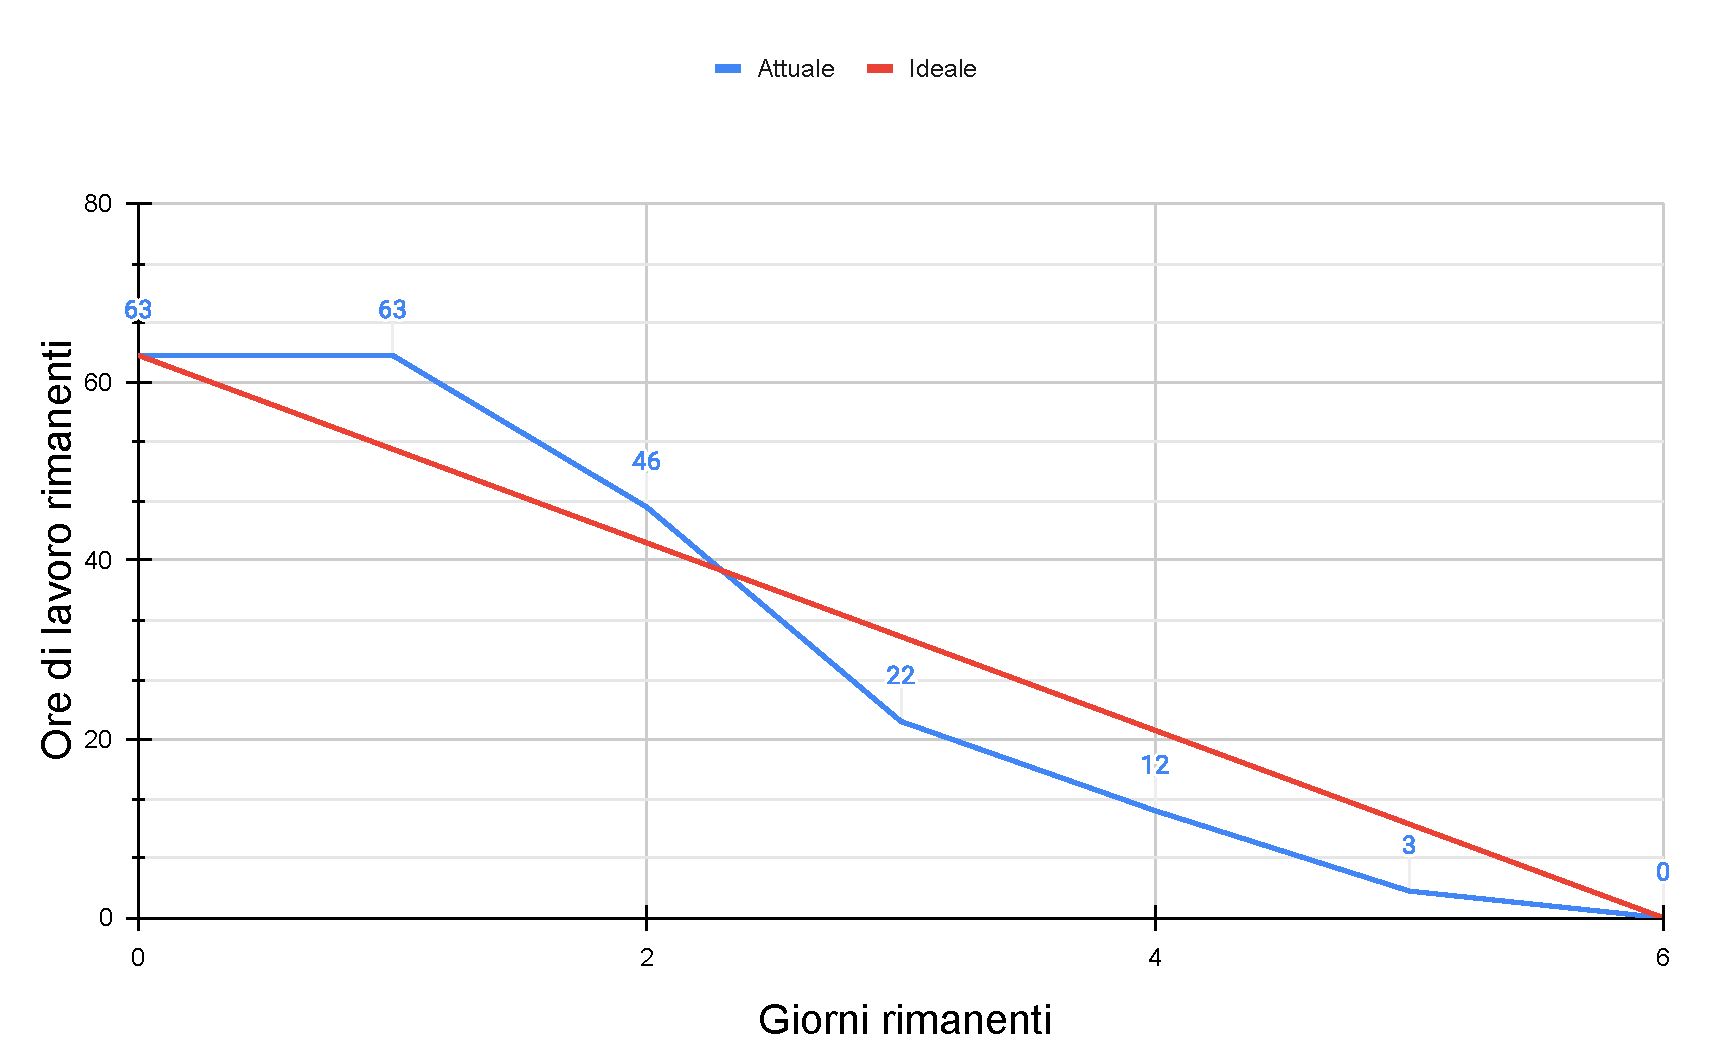
\includegraphics[trim= 0cm 0cm 0cm 0cm, clip, width=1\linewidth]{Deliverables/fourth-deliverable/img/BurndownChart.pdf}
    \caption{Burndown Chart Sprint \#$2$}
\end{figure}





